\documentclass[crop, tikz]{standalone}
\usetikzlibrary{decorations.markings}
\makeatletter

\begin{document}

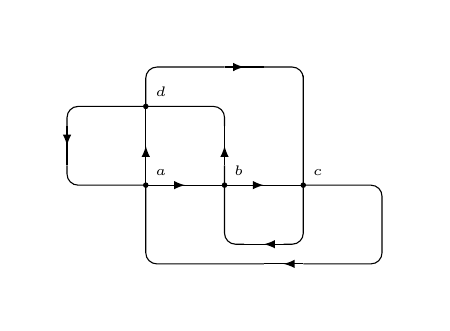
\begin{tikzpicture}[> = latex, font = \tiny]
	
	\begin{scope}[yscale = -1]

		\useasboundingbox (-2.5, 0) rectangle (2.5, 3.5);
	
		\node [above right] at (-1, 2) {$a$};
		\node [above right] at (0, 2) {$b$};
		\node [above right] at (1, 2) {$c$};
		\node [above right] at (-1, 1) {$d$};
		
		\foreach \x/\y in {-1/2, 0/2, 1/2, -1/1}
			\fill (\x, \y) circle (1 pt);
	
		\draw [rounded corners] (-0.5, 3) -- (-1, 3) -- (-1, 2) (-1, 1) -- (-1, 0.5) -- (-0.5, 0.5) -- (0, 0.5) (0.5, 0.5) -- (1, 0.5) -- (1, 0.75) -- (1, 2.75) --
			(0.75, 2.75) (0.25, 2.75) -- (0, 2.75) -- (0, 1.75) (0, 1.25) -- (0, 1) -- (-2, 1) -- (-2, 1.25) (-2, 1.75) -- (-2, 2) -- (-1, 2) (1, 2) -- (2, 2) -- (2, 3) --
			(1, 3) (0.5, 3) -- (-0.5, 3);
		
		\begin{scope}[decoration = {markings, mark = at position 0.5 with {\arrow{latex}}}]
			\draw [postaction = {decorate}] (-1, 2) -- (0, 2);
			\draw [postaction = {decorate}] (0, 2) -- (1, 2);
			\draw [postaction = {decorate}] (-2, 1.25) -- (-2, 1.75);
			\draw [postaction = {decorate}] (-1, 2) -- (-1, 1);
			\draw [postaction = {decorate}] (1, 3) -- (0.5, 3);
			\draw [postaction = {decorate}] (0, 0.5) -- (0.5, 0.5);
			\draw [postaction = {decorate}] (0.75, 2.75) -- (0.25, 2.75);
			\draw [postaction = {decorate}] (0, 1.75) -- (0, 1.25);
		
		\end{scope}
	
	\end{scope}

\end{tikzpicture}

\end{document}